\begin{frame}{Program}
    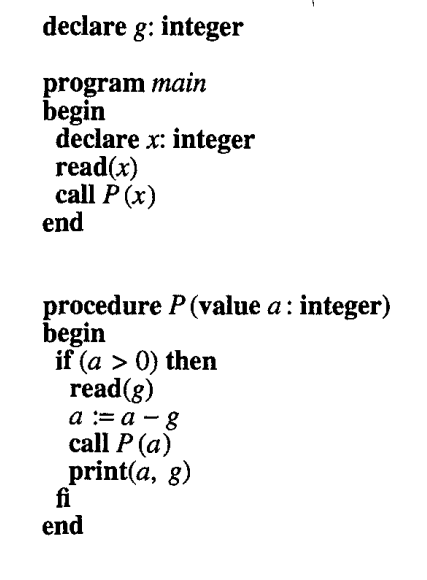
\includegraphics[height=0.7\paperheight, keepaspectratio]{images/program.png}    
\end{frame}

\begin{frame}{Supergraph}
    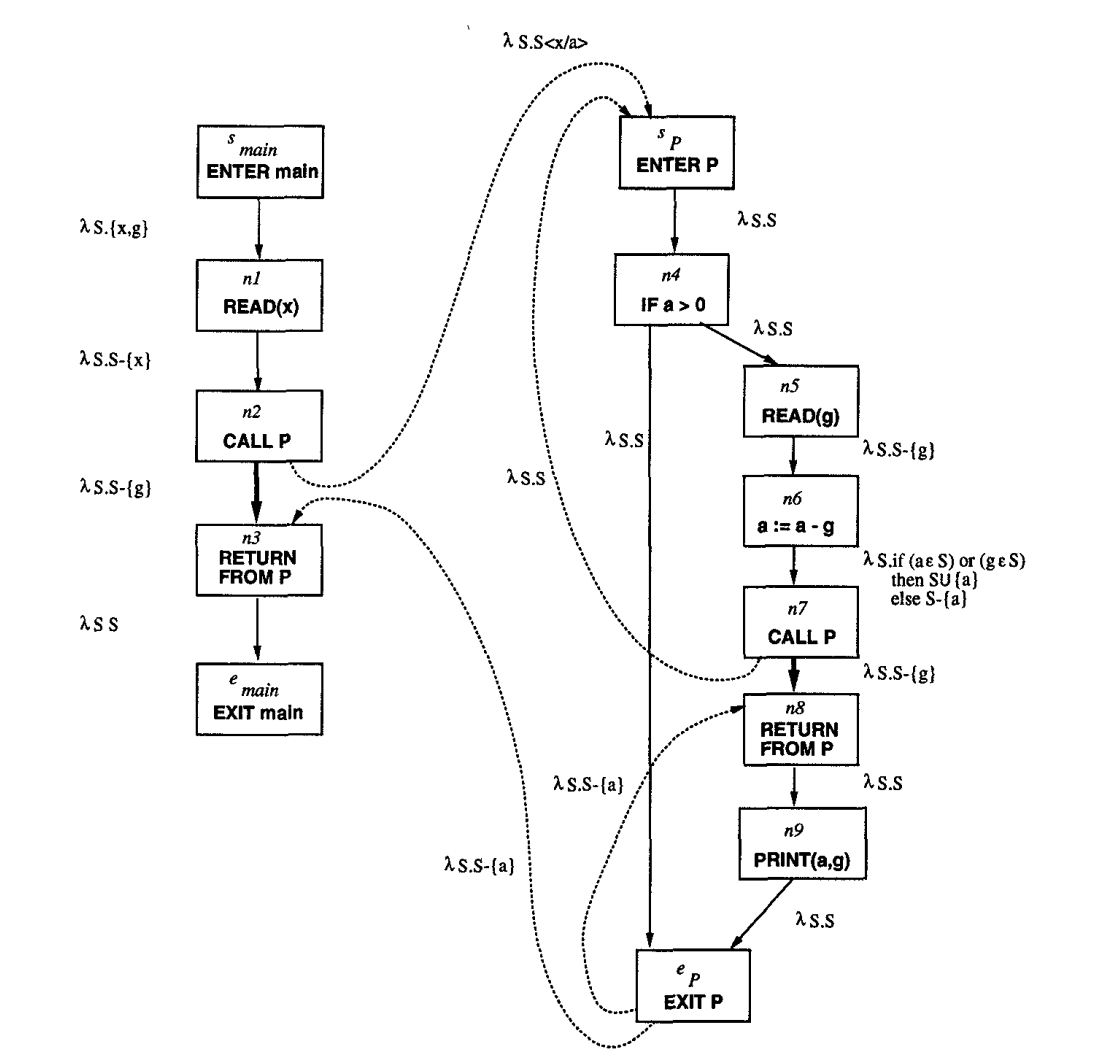
\includegraphics[height=0.79\paperheight, keepaspectratio]{images/supergraph.png}    
\end{frame}


\begin{frame}{Properties of representation relations}
  \begin{itemize}
    \item Interpretation $[[R]] : 2^D \to 2^D$ of a representation relation $R \subseteq (D \cup \{\mathbf{0}\}) \times (D \cup \{\mathbf{0}\})$:
    \[ [[R]] =_{\text{df}} \lambda X.(\{y \mid \exists x \in X.((x, y) \in R)\} \cup \{y \mid (\mathbf{0}, y) \in R\}) - \{\mathbf{0}\} \]
    \onslide<2>{
    \item Given a collection of functions $f_i : 2^D \to 2^D$ for $1 \le i \le j$,
    \[ f_1 \circ f_2 \circ \dots f_j = [[ R_{f_j} ; R_{f_{j-1}} ; \dots ; R_{f_1} ]]\]
    where the composition operation `;' on representation relations is defined as:
    \[ R_f \mathrel{;} R_g = \{(x,z)\in S\times S \mid \exists y\in S : (x,y)\in R_f \land (y,z)\in R_g\}. \]
    }
  \end{itemize}
\end{frame}

\tikzset{
  prog/.style={draw, rounded corners, minimum width=1.9cm, minimum height=0.45cm, fill=blue!10, font=\scriptsize, align=center},
  dot/.style={circle, fill, inner sep=1.8pt},
  cfgedge/.style={->, >=stealth, thick, black!75},
  initedge/.style={->, >=stealth, thick, red!80!black},
  normedge/.style={->, >=stealth, thick, blue!70!black},
  calledge/.style={->, >=stealth, thick, green!60!black},
  exedge/.style={->, >=stealth, thick, orange!90!black},
  legend/.style={font=\small\bfseries}
}

\newcommand{\drawprog}[4]{%
  \node[prog] (#1) at (#2, #3) {#4};
  \node[dot] (#1-0) at (#2+1.5, #3) {};
  \node[dot] (#1-x) at (#2+1.9, #3) {};
  \node[dot] (#1-y) at (#2+2.3, #3) {};
}

\newcommand{\skeleton}{%
  \drawprog{sm}{0}{0}{start main}
  \drawprog{x3}{0}{-1.2}{x = 3}
  \drawprog{p1}{0}{-2.4}{p()}
  \drawprog{rp}{0}{-3.6}{return from p}
  \drawprog{pr}{0}{-4.8}{printf(y)}
  \drawprog{em}{0}{-6.0}{exit main}

  \drawprog{sp}{6}{0}{start p()}
  \drawprog{iff}{6}{-1.2}{if ...}
  \drawprog{yx}{6}{-2.4}{y = x}
  \drawprog{p2}{6}{-3.6}{p()}
  \drawprog{rp2}{6}{-4.8}{return from p}
  \drawprog{pr2}{6}{-6.0}{printf(y)}
  \drawprog{ep}{6}{-7.2}{exit p}

  \node[legend] at (1.5, 0.55) {0};
  \node[legend] at (1.9, 0.55) {x};
  \node[legend] at (2.3, 0.55) {y};
}

\newcommand{\cfgedges}{%
  \draw[cfgedge] (sm.south)  -- (x3.north);
  \draw[cfgedge] (x3.south)  -- (p1.north);
  \draw[cfgedge] (p1.south)  -- (rp.north);
  \draw[cfgedge] (rp.south)  -- (pr.north);
  \draw[cfgedge] (pr.south)  -- (em.north);

  \draw[cfgedge] (sp.south)  -- (iff.north);
  \draw[cfgedge] (iff.south) -- (yx.north);
  \draw[cfgedge] (yx.south)  -- (p2.north);
  \draw[cfgedge] (p2.south)  -- (rp2.north);
  \draw[cfgedge] (rp2.south) -- (pr2.north);
  \draw[cfgedge] (pr2.south) -- (ep.north);

  \draw[cfgedge] (iff.west) -- ++(-1.5,0) |- (ep.west);
}

\newcommand{\initset}{%
  \draw[initedge] (sm-0) -- (x3-0);
  \draw[initedge] (sm-0) -- (x3-x);
  \draw[initedge] (sm-0) -- (x3-y);
}

\newcommand{\normAtXThree}{%
  \draw[normedge] (x3-0) -- (p1-0);
  \draw[normedge] (x3-y) -- (p1-y);
}

\newcommand{\normAtReturnFromP}{%
  \draw[normedge] (rp-0) -- (pr-0);
  \draw[normedge] (rp-x) -- (pr-x);
  \draw[normedge] (rp-y) -- (pr-y);
}

\newcommand{\normAtPrintfY}{%
  \draw[normedge] (pr-0) -- (em-0);
  \draw[normedge] (pr-x) -- (em-x);
  \draw[normedge] (pr-y) -- (em-y);
}

\newcommand{\normAtStartP}{%
  \draw[normedge] (sp-0) -- (iff-0);
  \draw[normedge] (sp-x) -- (iff-x);
  \draw[normedge] (sp-y) -- (iff-y);
}

\newcommand{\normAtIf}{%
  \draw[normedge] (iff-0) -- (yx-0);
  \draw[normedge] (iff-x) -- (yx-x);
  \draw[normedge] (iff-y) -- (yx-y);
}

\newcommand{\normAtYX}{%
  \draw[normedge] (yx-0) -- (p2-0);
  \draw[normedge] (yx-x) -- (p2-x);
  \draw[normedge] (yx-x) -- (p2-y);
}

\newcommand{\normAtRPT}{%
  \draw[normedge] (rp2-0) -- (pr2-0);
  \draw[normedge] (rp2-x) -- (pr2-x);
  \draw[normedge] (rp2-y) -- (pr2-y);
}

\newcommand{\normAtPRT}{%
  \draw[normedge] (pr2-0) -- (ep-0);
  \draw[normedge] (pr2-x) -- (ep-x);
  \draw[normedge] (pr2-y) -- (ep-y);
}

\begin{frame}{Supergraph}
\begin{center}
\begin{tikzpicture}[scale=0.7]
  \skeleton
  \cfgedges
  \onslide<2->{\initset}
  \onslide<2->{\normAtXThree}
  \onslide<2->{\normAtReturnFromP}
  \onslide<2->{\normAtPrintfY}
  \onslide<2->{\normAtStartP}
  \onslide<2->{\normAtIf}
  \onslide<2->{\normAtYX}
  \onslide<2->{\normAtRPT}
  \onslide<2->{\normAtPRT}
\end{tikzpicture}
\end{center}
\onslide<2->{%
  \small Initial fact is given as \(\{x,y\}\) . Hence, exploded edges are added (red) from
  \(\langle s_{\text{main}},0\rangle\) to \(\langle x{=}3,0\rangle\),
  \(\langle x{=}3,x\rangle\), \(\langle x{=}3,y\rangle\).
}
\end{frame}

\begin{frame}{Exploded Supergraph}
    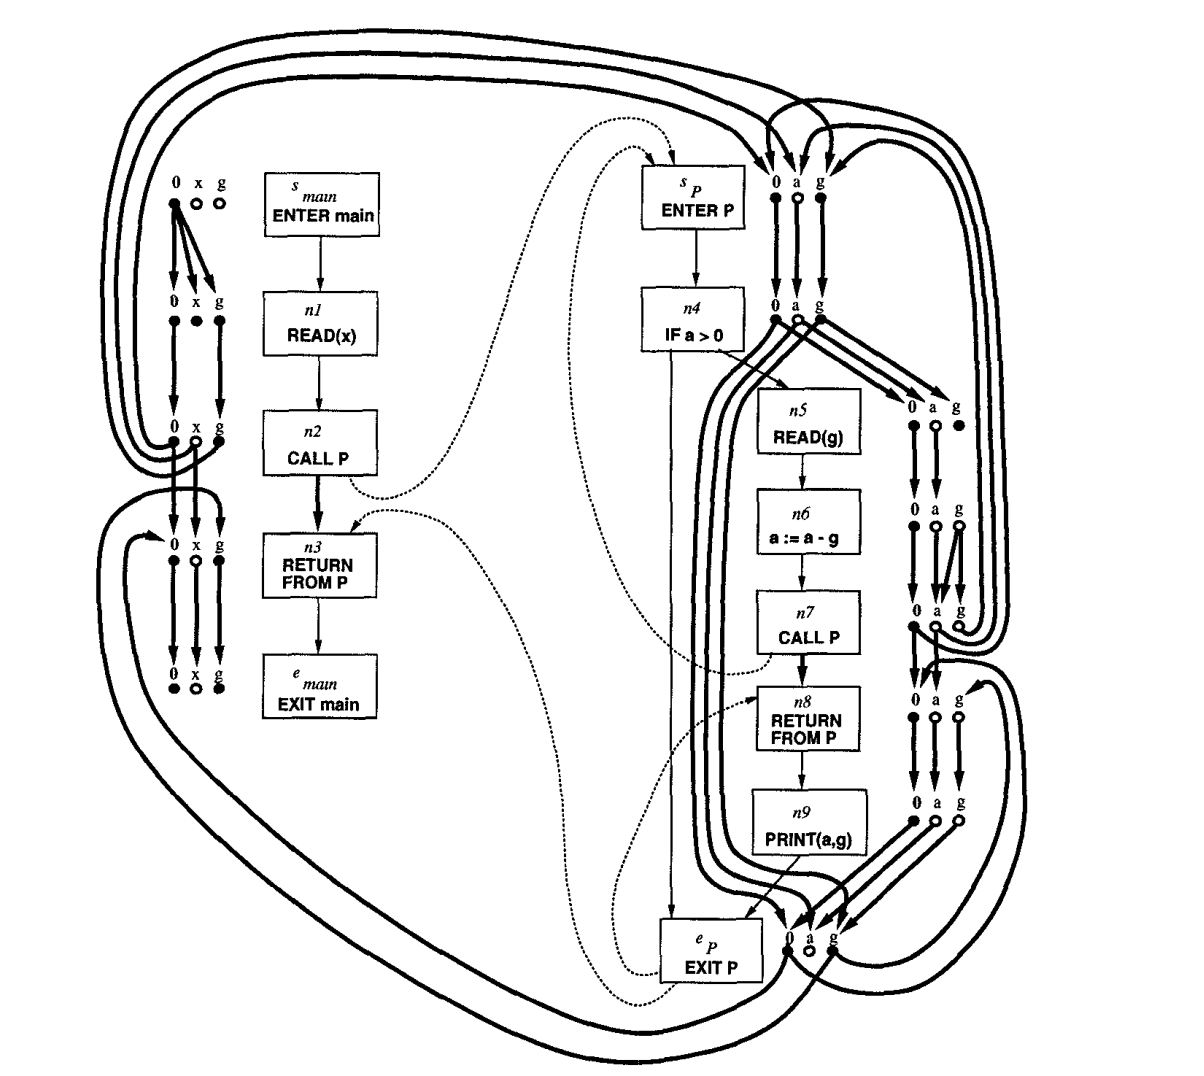
\includegraphics[height=0.79\paperheight, keepaspectratio]{images/exploded.png}    
\end{frame}

\begin{frame}{Property of exploded graph}
\textbf{Theorem 3.8 :} Given a super graph $G^*$ for an IFDS problem $IP$ with lattice $D$, and its corresponding exploded super graph $G^\#$, for any $d \in D$, $d \in JVP$ at node $n$ in $G^*$ \emph{iff} there is an \emph{interprocedurally valid} path from $\langle s_{main}, \mathbf{0} \rangle$ to $\langle n, d \rangle$ in $G^\#$. $\square$

\vspace{1em}
Follows from the property that for $1 \le i \le j$, 
$$f_1 \circ f_2 \circ \dots \circ f_j = [[R_{f_j}; R_{f_{j-1}}; \dots; R_{f_1}]].$$

\vspace{1em}
In other words, they have reduced dataflow analysis to graph reachability (along inter-procedurally valid paths).
\end{frame}